\documentclass{beamer}
\useoutertheme{infolines}
\usepackage[english]{babel}
\usepackage[latin1]{inputenc}
\usepackage[T1]{fontenc}
\usepackage{listings}
\usepackage{xspace}
\usepackage[super]{nth}
\usepackage{graphicx}
\lstset{language=Caml, basicstyle=\footnotesize,
  morekeywords={enum, alias, struct, union,
                asn1_alias, asn1_union, asn1_struct,
                UnknownVal, with_lwt, Exception}}

\newcommand{\PType}{$\mathcal{PT}$\hspace*{-.3ex}ype\xspace}
\newcommand{\PTypes}{$\mathcal{PT}$\hspace*{-.3ex}ypes\xspace}

\title[\url{https://github.com/ANSSI-FR/parsifal}]{Parsifal: writing efficient and robust binary parsers, quickly}
\author[O. Levillain]{\textbf{Olivier Levillain}, Herv� Debar and Benjamin Morin}
\institute[]{ANSSI / T�l�com Sud Paris}
\date{October \nth{23} 2013}

\begin{document}



%%%%%%%%%%%%%%%%%%%%%%%%%%%%%%%%%%%%%%%%%%%%%%%%%%%%%%%%%%%%%%%%%%%%%%%%%
\begin{frame}
  \maketitle
\end{frame}

\begin{frame}{Prerequisites for this tutorial}
  \begin{itemize}
  \item Linux system (tested on recent Debian or Ubuntu)
  \item an internet connection
  \item programming background
  \item (recommended) functional programming notions (ML/OCaml/Haskell)
  \end{itemize}

  \bigskip

  \uncover<2->{
    \begin{tabular}{l}
      apt-get install ocaml ocaml-findlib \\
      apt-get install liblwt-ocaml-dev \\
      apt-get install libcryptokit-ocaml-dev \\
      \\
      apt-get install git make \\
    \end{tabular}
  }
\end{frame}

\begin{frame}{Outline}
  \tableofcontents
\end{frame}



%%%%%%%%%%%%%%%%%%%%%%%%%%%%%%%%%%%%%%%%%%%%%%%%%%%%%%%%%%%%%%%%%%%%%%%%%
\section{Motivation}

\begin{frame}{Outline}
  \tableofcontents[currentsection]
\end{frame}

\begin{frame}{Origin of our work on parsers}
  In 2010, the EFF published datasets of IPv4 scans on port 443:
  \begin{itemize}
  \item 36~GB of raw data (180~GB when considering other sources)
  \item half of the answers are HTTPS... the rest can be exotic
  \item some servers do not behave according to the specifications
  \end{itemize}

  \medskip

  Our goal: analyse the data to understand what our browsers must deal with

  \medskip

  Existing TLS stacks did not meet our needs since they are either:
  \begin{itemize}
  \item limited (rejecting valid parameters)
  \item laxist (silently accepting invalid parameters)
  \item fragile (crashing on unexpected data)
  \end{itemize}

  \medskip

  For our study (a paper accepted at ACSAC 2012), we wrote a lot of
  tools using different languages.
\end{frame}

\begin{frame}{SSL/TLS: a brief tour of the messages}
  \begin{center}
    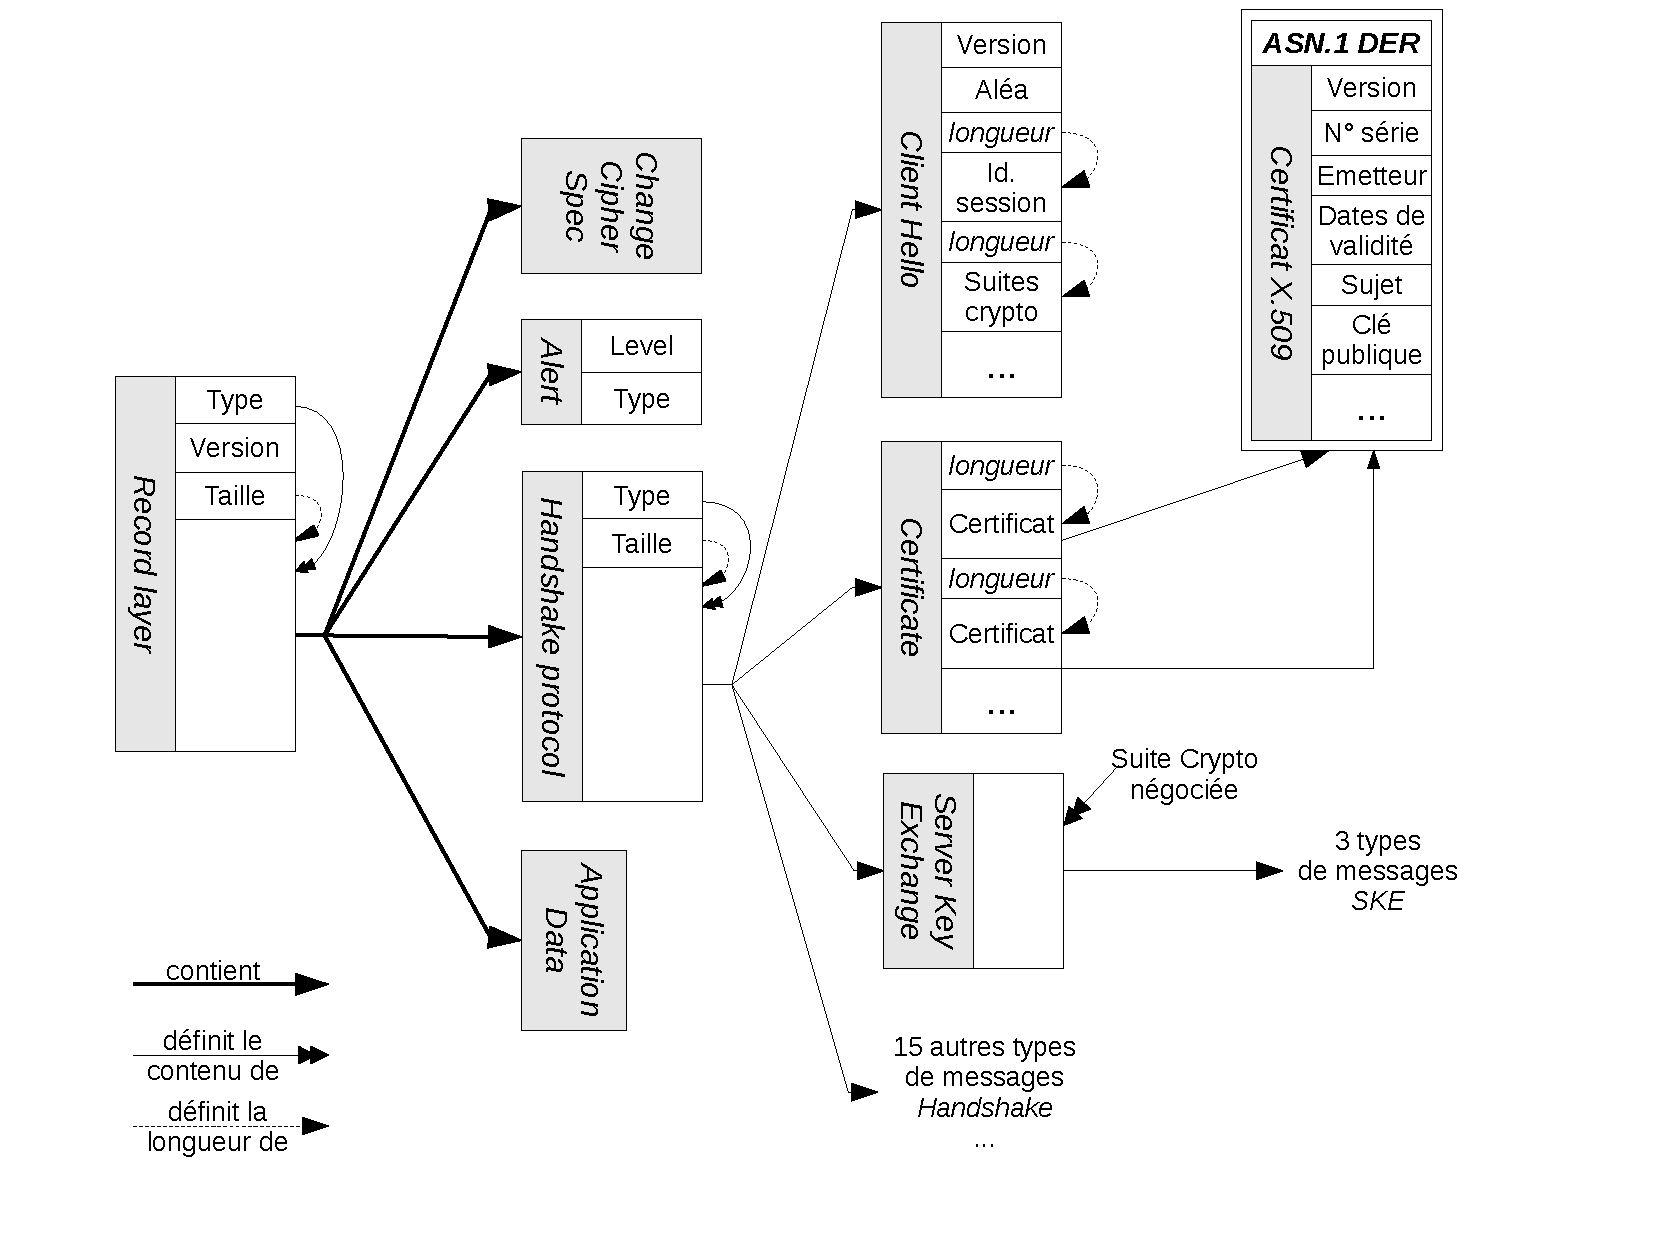
\includegraphics[width=.78\linewidth]{tls_messages}
  \end{center}
\end{frame}

\begin{frame}{Binary protocols/formats studied}
  Since 2011, we studied several formats:
  \begin{itemize}
  \item X.509 certificates
  \item SSLv2 and TLS messages
  \item BGP and MRT messages
  \item TAR archives (tutorial)
  \item DNS messages
  \item PE and PCI expansion ROM (UEFI)
  \item PNG and JPEG
  \item Kerberos
  \end{itemize}
\end{frame}

\begin{frame}{Where is the difficulty?}
  Protocol messages and file formats may be very complex to parse:
  \begin{itemize}
  \item variable length fields (TLS)
  \item context-dependent fields (DNS so-called compression)
  \item non-linear parsing (EXIF metadata)
  \item and a lot of tedious work that seems the same...
  \end{itemize}

  \medskip

  \uncover<2->{Question: how many ways can an integer be encoded?}
  \begin{itemize}
  \item<3-> big-endian / little-endian
  \item<4-> ASN.1 DER proposes three different ways (length, tag, integer value)
  \item<5-> Protobuf has a somewhat efficient bigint
  \item<6-> TAR uses octal strings (the \texttt{"101"} string means 65)
  \end{itemize}
\end{frame}

\begin{frame}{Parsers' expected properties}
  Our objective was multiple:
  \begin{itemize}
  \item analyse huge amounts of data to understand protocols:
    \begin{itemize}
    \item SSL data (using datasets like those of the EFF)
    \item BGP routing information (using RIS collectors)
    \end{itemize}
  \item write robust tools to detect anomalies
  \item normalise messages or files to remove vulnerabilities
  \end{itemize}

  \medskip

  To this purpose, the properties expected are:
  \begin{itemize}
  \item robustness
  \item efficiency
  \item ease of development
    \begin{itemize}
    \item expressive language
    \item concise code
    \item reusable code
    \end{itemize}
  \end{itemize}
\end{frame}

\begin{frame}{Demonstration}
  \begin{itemize}
  \item a tool used for our paper: \texttt{mapAnswers}
  \item grab and analyse certificates from an HTTPS server
  \item analyse a PCAP trace using \texttt{parsifal}
  \end{itemize}
\end{frame}


%%%%%%%%%%%%%%%%%%%%%%%%%%%%%%%%%%%%%%%%%%%%%%%%%%%%%%%%%%%%%%%%%%%%%%%%%
\section{Installation}

\begin{frame}{Outline}
  \tableofcontents[currentsection]
\end{frame}

\begin{frame}{Prerequisites (Debian/Ubuntu)}
  \begin{tabular}{l}
    apt-get install ocaml ocaml-findlib \\
    apt-get install liblwt-ocaml-dev \\
    apt-get install libcryptokit-ocaml-dev \\
    \\
    apt-get install git make \\
  \end{tabular}

  \bigskip

  Remarks:
  \begin{itemize}
  \item Debian Squeeze: patch needed...
  \item Debian Wheezy: OK
  \item Ubuntu Raring/Quantal: \texttt{universe} repository is needed
  \end{itemize}
\end{frame}

\begin{frame}{Downloading and compiling Parsifal}
  \begin{block}{GitHub repository}
    \tt
    \begin{tabular}{l}
      git clone https://github.com/ANSSI-FR/parsifal.git \\
      cd parsifal \\
    \end{tabular}
  \end{block}

  \uncover<2->{
    \begin{block}{Compilation and installation}
      \tt
      \begin{tabular}{l} 
        make \\
        LIBDIR=\$HOME/.ocamlpath BINDIR=\$HOME/bin make install \\
        export OCAMLPATH=\$HOME/.ocamlpath \\
        PATH=\$HOME/bin:\$PATH \\
      \end{tabular}
    \end{block}
  }

  \uncover<3->{
    \begin{block}{Installation check: grab and study some certificates}
      \tt
      \begin{tabular}{l} 
        mkdir tests \&\& cd tests \\
        probe\_server -H www.google.com extract-certs \\
        x509show -{}-subject *.pem \\
        x509show -{}-modulus *.pem \\
        x509show -g "**.distributionPoint" *.pem
      \end{tabular}
    \end{block}
  }
\end{frame}



%%%%%%%%%%%%%%%%%%%%%%%%%%%%%%%%%%%%%%%%%%%%%%%%%%%%%%%%%%%%%%%%%%%%%%%%%
\section{Parsifal's \PTypes}

\begin{frame}{Outline}
  \tableofcontents[currentsection]
\end{frame}


\begin{frame}{\PTypes}
  In Parsifal, a \PType consists of:
  \begin{itemize}
  \item an arbitrary OCaml type \texttt{t}
  \item a parsing function \texttt{parse\_t}
  \item a dumping function \texttt{dump\_t}
  \item a function producing a higher-level value \texttt{value\_of\_t}
  \end{itemize}

  \medskip

  \uncover<2->{
    There are three types of \PTypes:
    \begin{itemize}
    \item basic \PTypes (\texttt{uint8}, \texttt{string}, \texttt{list})
    \item constructed \PTypes, obtained using keywords and short descriptions
    \item custom \PTypes
    \end{itemize}
  }

\end{frame}


\begin{frame}[fragile]{Enumerations}
  RFC 5246 (TLSv1.2) encodes TLS version field using a 16-bit value.

{\footnotesize
\begin{lstlisting}
enum tls_version (16, UnknownVal UnknownVersion) =
  | 0x0002 -> SSLv2
  | 0x0300 -> SSLv3
  | 0x0301 -> TLSv1
  | 0x0302 -> TLSv1_1
  | 0x0303 -> TLSv1_2
\end{lstlisting}
}

\end{frame}


\begin{frame}{SSL/TLS: describing alert messages}
  \begin{center}
    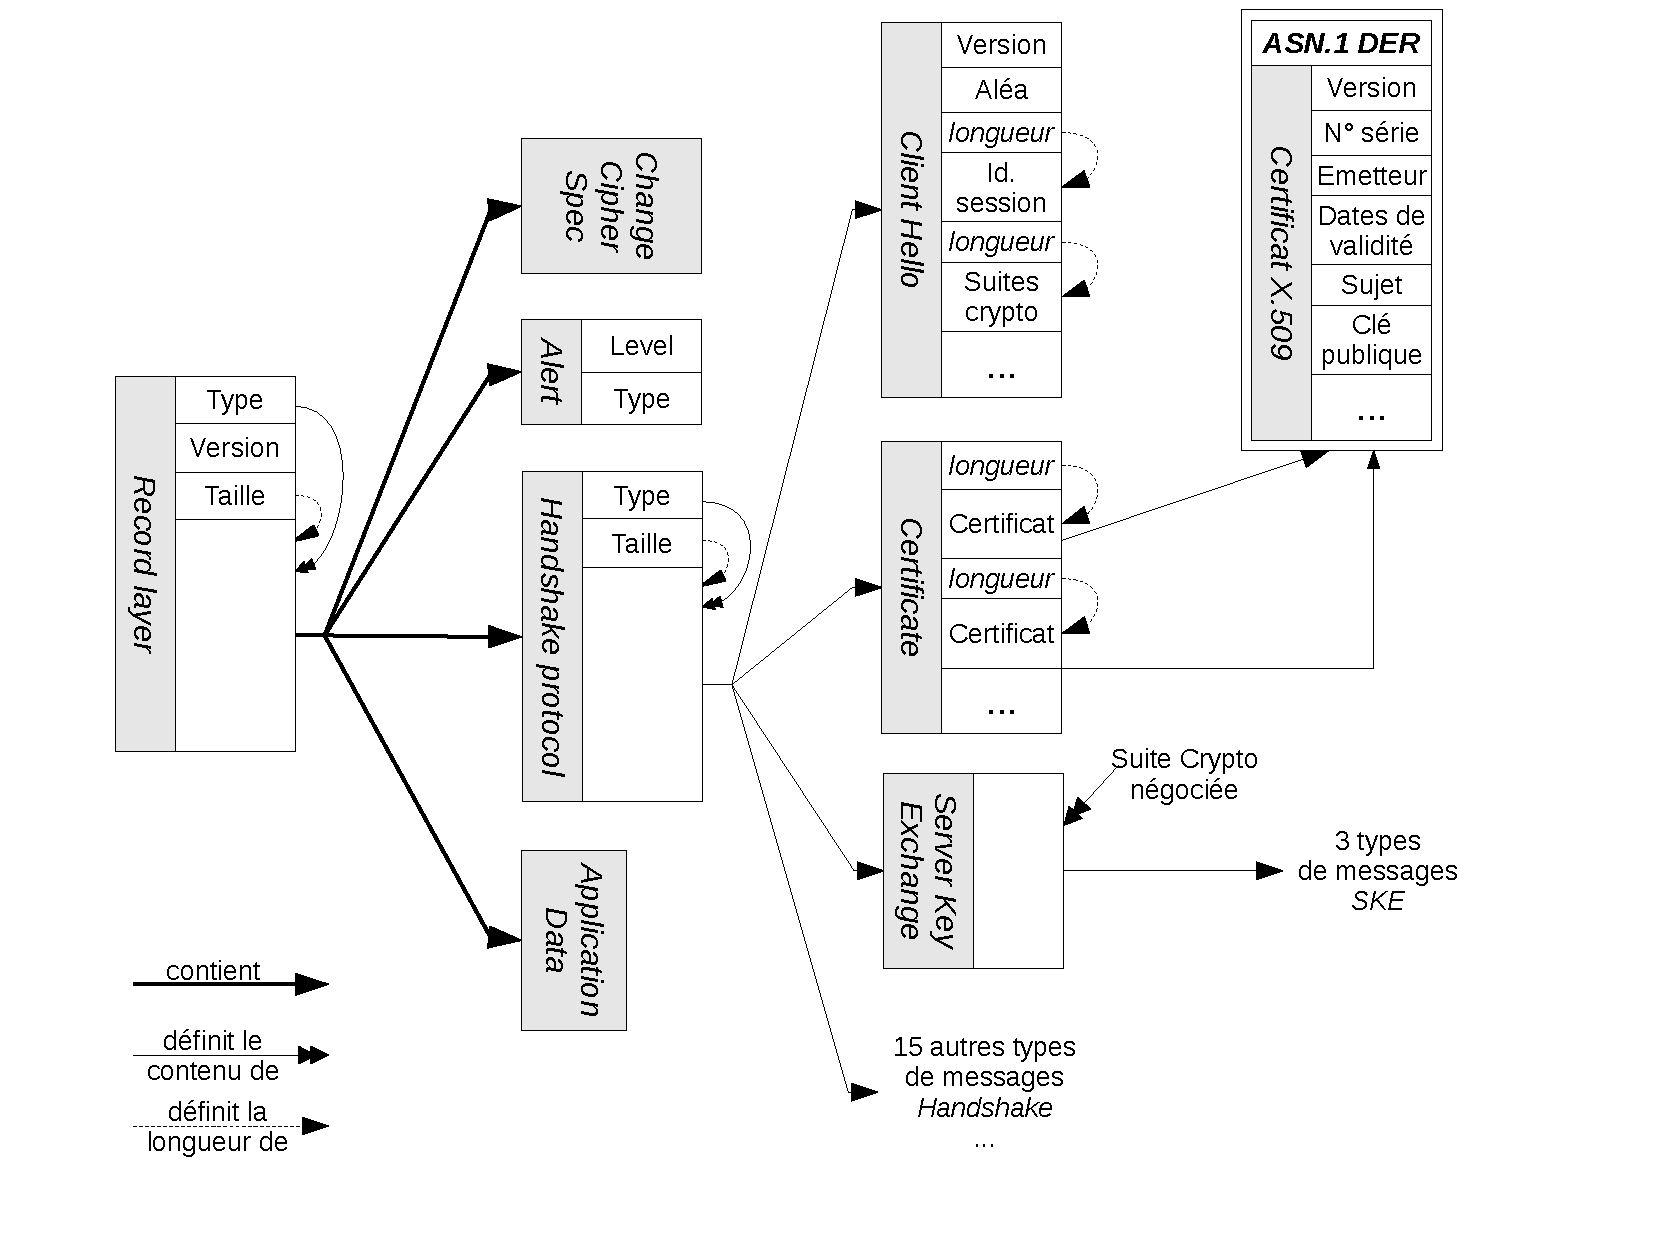
\includegraphics[width=.78\linewidth]{tls_messages}
  \end{center}
\end{frame}


\begin{frame}[fragile]{Structures (1/2)}
  RFC 5246 (TLSv1.2) extract:
{\footnotesize
\begin{lstlisting}
enum { warning(1), fatal(2), (255) } AlertLevel;

enum {
    close_notify(0),
    unexpected_message(10),
     ...
    unsupported_extension(110),
    (255)
} AlertDescription;

struct {
    AlertLevel level;
    AlertDescription description;
} Alert;
\end{lstlisting}
}
\end{frame}


\begin{frame}[fragile]{Structures (2/2)}
  Parsifal implementation:
{\footnotesize
\begin{lstlisting}
enum tls_alert_level (8, Exception) =
  | 1 -> Warning
  | 2 -> Fatal

enum tls_alert_type (8, UnknownVal UnknownAlertType) =
  | 0 -> CloseNotify
  | 10 -> UnexpectedMessage
    ...
  | 110 -> UnsupportedExtension

struct tls_alert =
{
  alert_level : tls_alert_level;
  alert_type : tls_alert_type
}
\end{lstlisting}
}
\end{frame}


\begin{frame}{SSL/TLS: handshake messages depend on a type}
  \begin{center}
    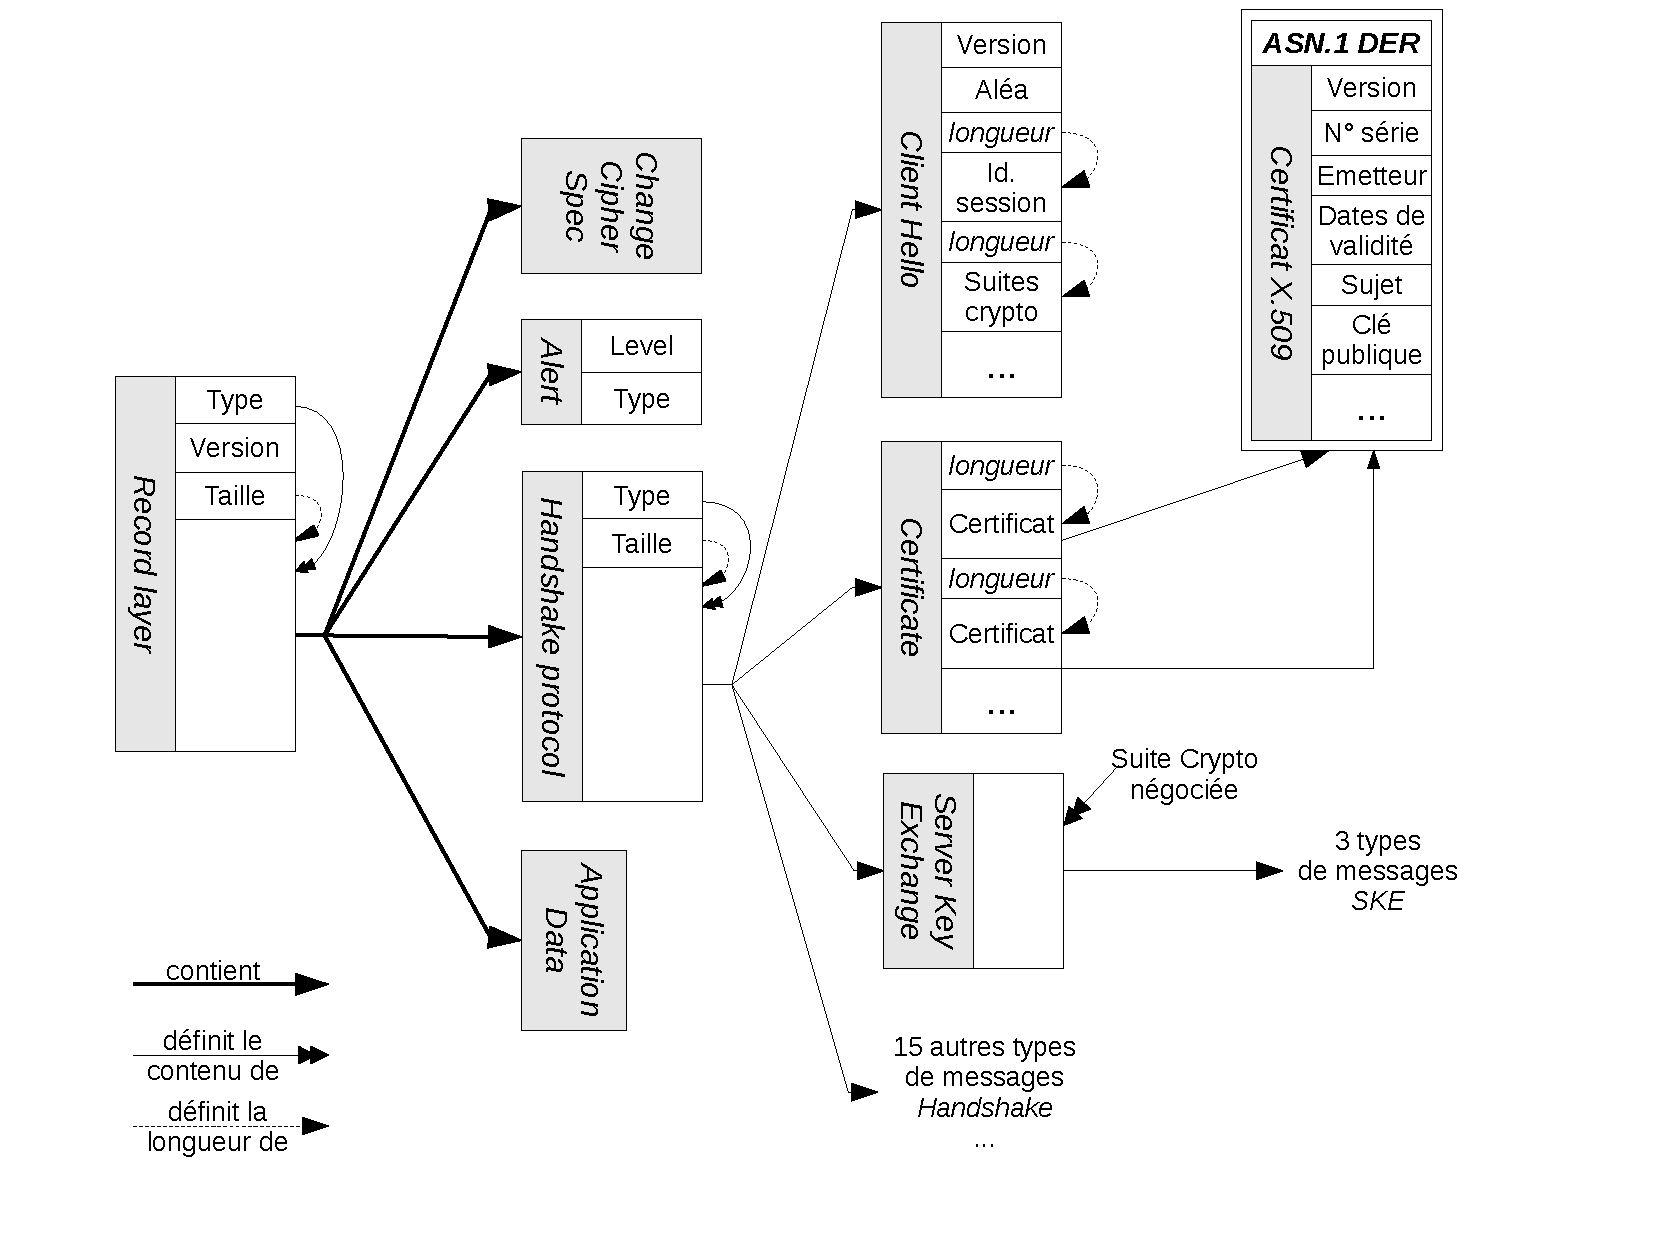
\includegraphics[width=.78\linewidth]{tls_messages}
  \end{center}
\end{frame}


\begin{frame}[fragile]{Unions}
  Supposing \texttt{client\_hello} and \texttt{server\_hello} have
  been written, we can write:

{\footnotesize
\begin{lstlisting}
enum hs_message_type (8, UnknownVal HT_Unknown) =
  | 1 -> HT_ClientHello
  | 2 -> HT_ServerHello
  | ...

union handshake_content [enrich] (Unparsed_HSContent) =
  | HT_ClientHello -> ClientHello of client_hello
  | HT_ServerHello -> ServerHello of server_hello
  | ...

struct handshake_msg = {
  handshake_type : hs_message_type;
  handshake_content : container[uint24] of
                         handshake_content(handshake_type)
}
\end{lstlisting}
}

\end{frame}


\begin{frame}{Other constructions}
  \begin{itemize}
  \item \texttt{containers} (base64, ASN.1 encapsulations)
  \item \texttt{asn1\_union} and \texttt{asn1\_struct}
  \item \texttt{struct} may contain bit fields
  \end{itemize}
\end{frame}






%%%%%%%%%%%%%%%%%%%%%%%%%%%%%%%%%%%%%%%%%%%%%%%%%%%%%%%%%%%%%%%%%%%%%%%%%
\section{PNG tools}

\begin{frame}{Outline}
  \tableofcontents[currentsection]
\end{frame}

\begin{frame}[fragile]{PNG 101: a list of chunks}
  A PNG has the following structure:
  \begin{itemize}
  \item a magic string identifying the format (\verb+"\x89PNG\r\n\x1a\n"+)
  \item a list of chunks
  \end{itemize}

  \medskip

  Each chunk contains:
  \begin{itemize}
  \item the chunk size (on a big endian 32 bits)
  \item the chunk type (a 4 character string)
  \item the chunk data (whose length was given earlier)
  \item a checksum (a CRC32)
  \end{itemize}
\end{frame}

\begin{frame}{Our first project}
  \tt
  \begin{tabular}{l} 
    cd parsifal \\
    ./mk\_project pngtools \\
    cd pngtools \\
    make \\
    ./pngtools
  \end{tabular}
\end{frame}

\begin{frame}{Let's implement PNG, one step at a time}
  \begin{itemize}
  \item Write a program checking the magic string
  \item<2-> Add support for chunks
  \item<3-> Simple tool to print the chunk types
  \item<4-> Chunk Filter: only keep critical chunks
  \item<5-> First custom \PType: \texttt{crc\_check}
  \item<6-> First union to enrich chunk content
  \item<7-> ...
  \end{itemize}
\end{frame}

\begin{frame}{Conclusion on PNG}
  
  \begin{itemize}
  \item step by step description of the PNG format
  \item basic validation of the structure
  \item possibility to add checks
  \item such a validation/sanitisation would thwart some known
    vulnerabilities on \texttt{libpng}:
    \begin{itemize}
    \item CVE-2011-0408
    \item CVE-2008-1382
    \item CVE-2007-5266
    \item CVE-2007-2445
    \item CVE-2004-0597
    \item ...
    \end{itemize}
  \end{itemize}
\end{frame}



%%%%%%%%%%%%%%%%%%%%%%%%%%%%%%%%%%%%%%%%%%%%%%%%%%%%%%%%%%%%%%%%%%%%%%%%%
\section{A CSR validator}

\begin{frame}{Outline}
  \tableofcontents[currentsection]
\end{frame}

\begin{frame}[fragile]{Null characters in Common Names}

  In 2009, Moxie Marlinspike showed an attack on Certificate Signing
  Requests:
  \begin{itemize}
  \item a CSR is submitted for \verb+www.mybank.com\x00.attacker.com+
  \item the Certification Authority thinks the signed domain is under \texttt{attacker.com}
  \item most TLS clients (written in C) stop at the first null character
  \item CVE-2009-2408
  \end{itemize}

  \medskip

  Recently, a similar vulnerability has resurfaced in different languages:
  \begin{itemize}
  \item python (CVE-2013-4238 and) 
  \item ruby (CVE-2013-4073)
  \end{itemize}
\end{frame}

\begin{frame}[fragile]{CSR specification}
  Let's start from the RFC 2314 (PKCS\#10):
{\footnotesize
\begin{lstlisting}
CertificationRequestInfo ::= SEQUENCE {
  version Version,
  subject Name,
  subjectPublicKeyInfo SubjectPublicKeyInfo,
  attributes [0] IMPLICIT Attributes }

Version ::= INTEGER

Attributes ::= SET OF Attribute

CertificationRequest ::= SEQUENCE {
  certificationRequestInfo CertificationRequestInfo,
  signatureAlgorithm SignatureAlgorithmIdentifier,
  signature Signature }

SignatureAlgorithmIdentifier ::= AlgorithmIdentifier

Signature ::= BIT STRING
\end{lstlisting}
}
\end{frame}

\begin{frame}[fragile]{Parsifal implementation}
  Most of the fields have already been implemented for X.509
  certificates:
{\footnotesize
\begin{lstlisting}
asn1_struct certificationRequestInfo = {
  version : der_smallint;
  name : distinguishedName;
  subjectPublicKeyInfo : subjectPublicKeyInfo;
  attributes : der_object;
}

asn1_struct certificationRequest = {
  certificationRequestInfo : certificationRequestInfo;
  signatureAlgorithm : algorithmIdentifier;
  signatureValue : bitstring_container of signature(signatureType_of_algo signatureAlgorithm)
}
\end{lstlisting}
}
\end{frame}

\begin{frame}{Some checks on CSR}
Now we have a (partial) description of a CSR, we may want to check
\begin{itemize}
\item the RSA signature
\item that the subject does not contain any null character
\end{itemize}
\end{frame}

\begin{frame}{Conclusion on CSRs}

\begin{itemize}
\item Parsifal can help reuse code very easily
\item ASN.1 structures can be described very quickly using 
\item this kind of robust validator could be used in front of real
  applications, to drop invalid requests early in the process
\end{itemize}
\end{frame}



%%%%%%%%%%%%%%%%%%%%%%%%%%%%%%%%%%%%%%%%%%%%%%%%%%%%%%%%%%%%%%%%%%%%%%%%%
\section{Parsifal: past, present and future}

\begin{frame}{Outline}
  \tableofcontents[currentsection]
\end{frame}


\begin{frame}{Conclusion}
  Past:
  \begin{itemize}
  \item since 2011, some protocols and file formats described
  \item Parsifal tools used to analyse SSL/TLS data
  \end{itemize}

  \medskip

  Present:
  \begin{itemize}
  \item work in progress on PNG and JPEG files
  \item CSR and certificate validation
  \end{itemize}

  \medskip

  Future:
  \begin{itemize}
  \item write a complete SSL/TLS stack using Parsifal
  \item more challenges?
  \item if you are interested, please tell me, and eventually contribute!
  \end{itemize}
\end{frame}



\begin{frame}{Questions?}
  \vspace*{\stretch{1}}

  \begin{center}
    Thank you for your attention.

    \bigskip
 
    \url{https://github.com/ANSSI-FR/parsifal}   

    \medskip

    \texttt{olivier.levillain@ssi.gouv.fr}
  \end{center}

  \vspace*{\stretch{1}}
\end{frame}


\end{document}
